\chapter{Face Recognition}
\label{sec:facerec}

As previously mentioned, a face recognition system embedded on the customer's platform would extract metadata that could be interesting for our recommendation engine and valuable for the user experience.

We will first highlight how our use case is different from the general case, then present how face recognition is usually tackled, and finally explore our system currently in production. We will emphasize our contributions: a new metric-learning loss function, the threshold-softmax loss, and a study of several methods for exploiting unlabeled faces during training.

\subsection{Industrial setting}

In our industrial setting, we wish to identify some people of interest ("VIPs") among many unknown people in videos with unconstrained facial pose, illumination, expression and occlusion. The set of identities of interest is known ahead of time but a lot of the input pictures, if not most, are unknown people that must be rejected by the system. This particular setting makes this an instance of a subject-dependent open-set protocol, which we observe to be an understudied case, not even considered in Wang et al (2021) \cite{survey} (Figure \ref{fig:survey}).

We believe this setting is particularly common under some industrial settings in which we are interested in some people, like celebrities, for which we can acquire datasets if needed, among many unknown test-time distractors. One such example would be reidentifying famous YouTubers in fan compilations, clips or video reuses. Another would be to reidentify famous actors in movies among extras.

We call \emph{distractors} faces whose identity is unknown to the system. It is expected that the system rejects those faces and is aware that they are unknown. The presence or absence of distractors is what differentiates open-set and close-set settings.

Hexaglobe's Face Recognition system has some specificities compared to the algorithms laid in the literature:

\begin{enumerate}
    \item Contrarily to most, this work is focused on identifying a known set of identities among distractors. Most works instead deal with verifying if a query face is the same person as a key face, for instance, verifying if the person at the customs is the same as the one on the passport being presented.
    
    \item Most works on classifiers focus on having a correct best guess, but this system does not have to make a prediction for every input. The model rejecting some inputs because of uncertainty is a better outcome than a failed prediction. Knowing that we don't know is crucial here.

    \item Our work is deployed at scale where it analyzes hundreds of user uploaded videos per day. Those videos present real world faces in the wild, with occlusions, variable lighting conditions, image resolution, quality and scale, not properly aligned, sometimes with extreme facial poses, making this data more challenging than most used datasets currently used in publications \citep{celeb1m}.
\end{enumerate}

However, our setting allows some relaxations :

\begin{enumerate}
    \item As a public video platform using the system for tagging videos with identities for search improvements, we are only interested in tagging the most popular people. These people can be decided ahead of time and our problem becomes a semi-open set face recognition problem: the set of identities to recognize is known ahead of time but there are unknown distractors to reject.

    \item All errors are not equal. It is more harmful to add a wrong tag than to miss one. In our case, precision is more important than recall. This makes it possible, even needed, to let the model express its lack of confidence and not act on uncertain predictions.

    \item As we are interested in overall video tagging and not per frame tagging, per frame errors are not harmful if they can be smoothed out.
\end{enumerate}

Besides, considering the volume of existing videos (approx 8M) and the number of new uploads per day, processing a video should not take more than 5 minutes. In order to guarantee this processing time, we extract 300 frames evenly spaced throughout the video.

Finally, as our system is meant to have a quickly growing set of persons of interest, we favor fast iterations, both in model training time and time needed to add a subject to the set of known persons.

\section{Standard systems}

Face recognition (FR) systems based on deep learning have been under heavy research these past years. As outlined in Wang et al (2021) \cite{survey}, FR systems can be characterized by two major features: whether we expect the train and test sets to contain the same identities or not (subject-dependent vs subject-independent protocol), and the evaluation task: verification (whether a picture matches the identity of another), closed-set identification (all input test identities are known to the system) and open-set identification (some test inputs does not belong to any known identity and must be rejected).

We observe that a lot of work went into the subject-independent closed-set protocol thanks to MegaFace \cite{megaface}. Contrarily, the subject-dependent protocol has mostly been considered in the closed-set evaluation and deemed to be solved with a simple image classifier, not receiving much attention. Figure \ref{fig:survey} does not even consider other settings.

\begin{figure}
    \centering
    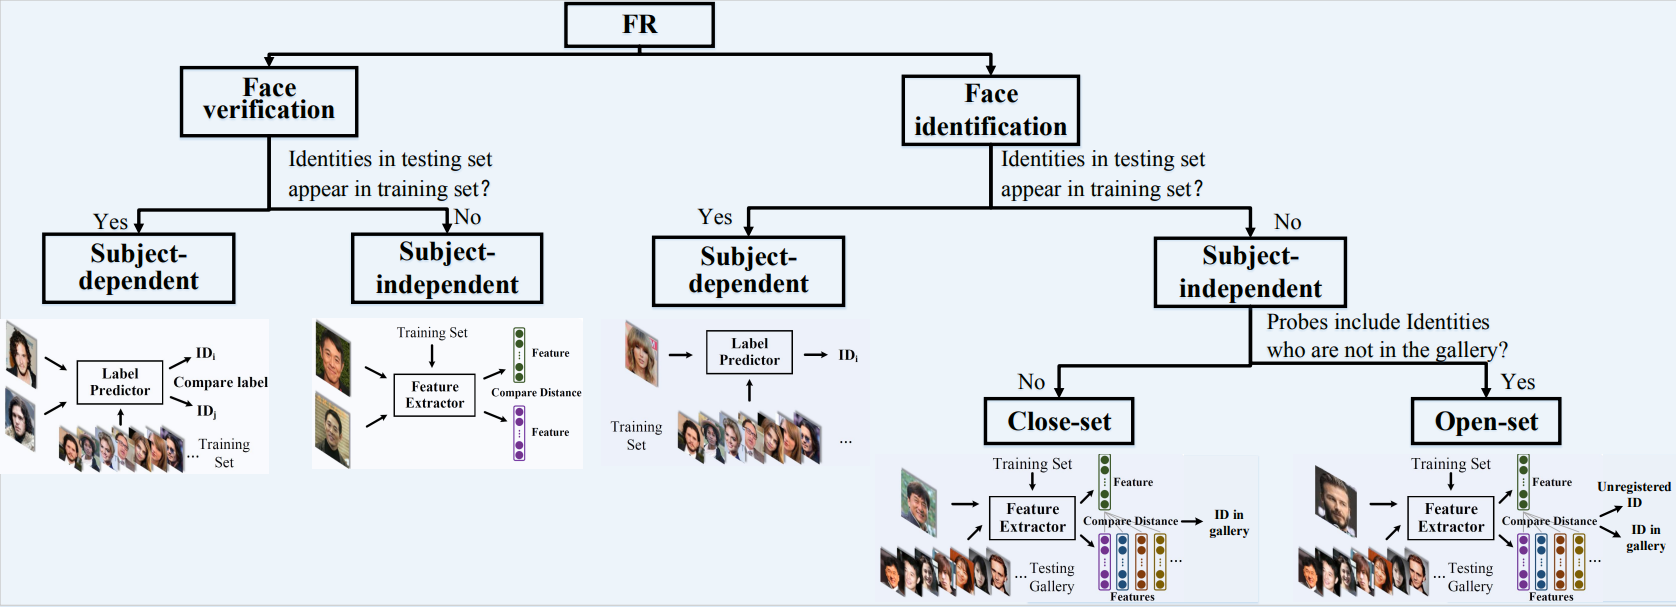
\includegraphics[width=\columnwidth]{50-files/survey.png}
    \caption{Figure 17 from Wang et al (2021) \cite{survey}. The comparison of different training protocol and evaluation tasks in FR. In terms of training protocol, FR can be classified into subject-dependent or subject-independent settings according to whether testing identities appear in training set. In terms of testing tasks, FR can be classified into face verification, close-set face identitification, open-set face identification.}
    \label{fig:survey}
\end{figure}

\subsection{Open-set/closed-set and subject-dependent/subject-independent recognition}

As explicited in Figure \ref{fig:survey}, face recognition systems, when focusing on the task of open-set verification, have to decide whether two pictures of people unseen during training time are the same person or not. In order to generalize to unseen identities, the systems are trained under a similarity learning objective to produce dense semantic face representations that should be similar for same identities and dissimilar for different identities under cosine or Euclidean distance (for the general case). The Triplet Loss \cite{triplet,triplet-face} explicitly enforces those properties with a negative and positive pair relative to an anchor face. While it marked the beginning of scalable face recognition systems, the long training time drove the community to more data-efficient and time-efficient techniques. Present state-of-the-art approaches such as SphereFace \cite{sphereface}, CosFace \cite{cosface}, ArcFace \cite{arcface}, AdaCos \cite{adacos} mostly build on classification losses such as Cross-Entropy with margin and representation constraints (such as normalizing L2 norm). Current datasets  for those approaches have about 10k of identities in order to learn good discriminative features that generalize well (Megaface \cite{megaface}, VGGFace2 \cite{vggface2}, MS1M \cite{celeb1m}, ImdbFace \cite{imdbface}, IJB-{A,B,C} \cite{ijb-a, ijb-b, ijb-c}).

Those representations are then extracted from reference images and compared independently with the input image’s representation.

\begin{figure}
    \centering
    \includegraphics[width=\columnwidth]{50-files/facerec1.pdf}
    \caption{Training of classification-based metric learning algorithm. The algorithm is trained to classify faces in different identities, with a margin in softmax and representation constraints.}
    \label{fig:facerec1}
\end{figure}

\begin{figure}
    \centering
    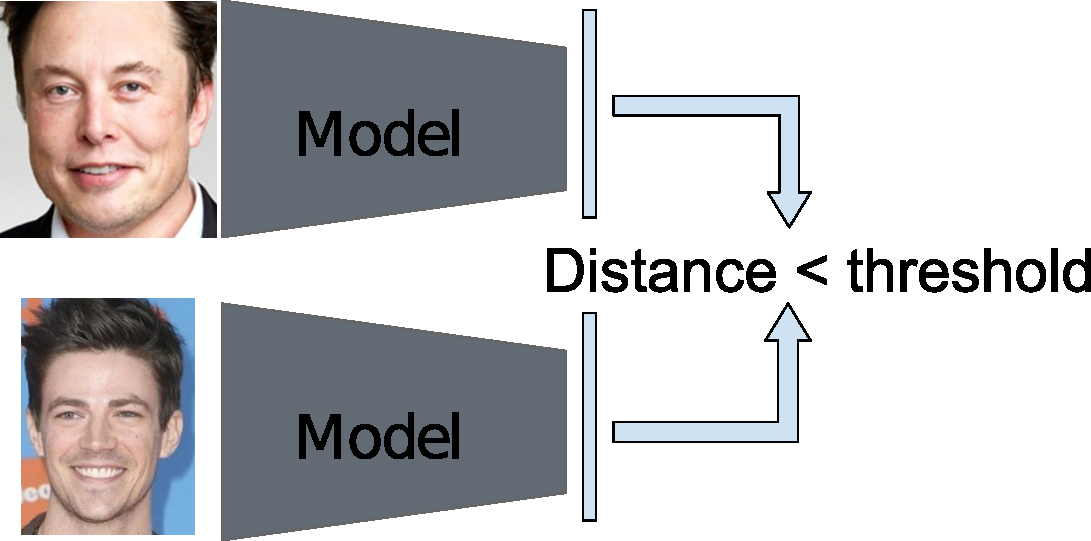
\includegraphics[width=\columnwidth]{50-files/facerec2.pdf}
    \caption{Test time usage of feature vectors. Two images’ representations are compared under a distance metric. A distance under a predefined threshold indicates the same identity.}
    \label{fig:facerec2}
\end{figure}

When tasked to identify, the input image (the “probe”) is encoded in a feature vector and compared to all the encoded reference picture vectors (the “gallery”), aiming for minimum distance on the correct identity. This strategy has some shortcomings outlined in \cite{ijb-a}: it is unclear how to aggregate various feature vectors from several images of the same identity, and current systems are not precise enough to reject all the images in the gallery for unknown probe identity when the gallery has many pictures, triggering false detections. For testing, LFW \cite{lfw} is a common test set as well.

\section{Metric learning}

In order to generalize to unseen faces, FR systems are usually seen as a metric learning (or similarity learning) problem instance. In general, metric learning aims to learn an embedding space that is semantically meaningful wrt to a chosen distance function (usually euclidean or angular).

Under this framework, we aim to obtain a neural network embedding a face into similar vectors for the same person and dissimilar vector for different people. The similarity measure is often euclidean or angular.

\subsection{Triplet loss}

The most direct translation of this goal is the Triplet Loss \citep{triplet-face,tripletloss,triplet}. For a neural net $f$ that takes a face as an input and outputs a vector, and a distance function $d$, we want to minimize

\begin{equation}
    \mathcal{L} = d(f(A_i), f(A_j)) - d(f(A_i), f(B_k))
\end{equation}

where $A_i$ and $A_j$ are two different pictures of a person A, and $B_k$ is a picture of a different person B.

While this work, this requires a lot of time to converge.

\subsection{Softmax}

Posing the problem as a classification task allows to leverage the efficiency of the cross-entropy loss and the discriminative capability of neural networks. In order to frame $f$ as a classifier, we need to define

\begin{equation}
    h(x) = \text{softmax}(f(x) \cdot W^T)
\end{equation}

Here, $W$ is a learnable $k\times d$ matrix where $k$ is the number of identities to classify and $d$ is the dimension of the embedding row vector produced by $f$. The $i$th row of $W$ can be interpreted as the prototypical embedding for class $i$.

At inference time, $W$ is discarded and a distance function is used to compare the embeddings. It is hoped that $f$ was trained on enough identities in order to make a rich, semantically meaningful vector space. During training, as the embeddings were discriminated with a linear classifier, a parameter-free distance function should be able to discriminate embeddings from people not seen during training.

\subsection{L2-softmax}
\newcommand{\vnorm}[1]{\langle #1 \rangle}

Vanilla softmax has some notable drawbacks: it does not enforce positive pairs to remain together and negative pairs further; it is biased towards the training distribution unbalance; and uncertain samples produce decisions with low confidence that are poorly penalized.

\citet{l2softmax} (Figure \ref{fig:tsm}a) proposes to fix all of those by enforcing a L2 constraint on both the output vector of $f$ and each row of $W$. Instead of maximizing the softmax output with maximum inner product between the correct row of $W$ and $f(x)$, this aims to maximize (minimize) the cosine similarity between the correct (incorrect) row of $W$ and $f(x)$. If we accept the notation $\vnorm{n}$ for a matrix $n$ with each row vector normalized to unit length, the L2-softmax is:

\begin{equation}
    \label{eq:l2sm}
    h(x) = \text{softmax}(s \vnorm{f(x)} \cdot \vnorm{W}^T ) = \text{softmax}(s \cos(f(x), W)) = \text{softmax}(s \cos \theta)
\end{equation}

where the scalar $s$ can be either interpreted as a radius or the temperature of the softmax. The higher the $s$, the more the softmax will resemble a hard $\text{argmax}$. As $\cos$ is bounded in [-1; 1], it is necessary to control the sharpness of the softmax with a temperature in order to control the gradient magnitude. $\theta$ is the vector of the angles between $f(x)$ and each row of $W$.

Note that in the equation above, $\cos$ is applied independently to each row of $W$ and $f(x)$, also making $\theta$ a vector of size $k$ representing the angles between $f(x)$ and each row of $W$.

\subsection{ArcFace}

ArcFace \cite{arcface} (Figure \ref{fig:tsm}b) builds on this by enforcing a margin between classes. The L2-softmax (Eq. \ref{eq:l2sm}) emits a valid high probability as soon as $f(x)$ has its smallest angle with the prototype of the correct class in $W$. They thought this was not enough and wanted to add another guarantee, that small perturbations to $f(x)$ due to input distribution shifts or hard samples would not be predicted as another class. As such, they add an hyperparameter margin $m$ in the equation to repel the embedding by $m$. By adding $m$ radians to the angle of the correct class the angular distance with other classes is forced to be greater than the margin:

\begin{equation}
    h(x) = \text{softmax}(s \cos(\theta + m\hat{y}))
\end{equation}

where $\hat{y}$ is a $k$ dimensional row vector one-hot encoding the target class.

Some other margins were proposed prior to ArcFace such as \citep{sphereface} or \citep{cosface} but showed lesser accuracy at test time.

\section{\arr \emph{Contribution}: Threshold-Softmax}

\subsection{Principle}

\begin{figure}
    \centering
    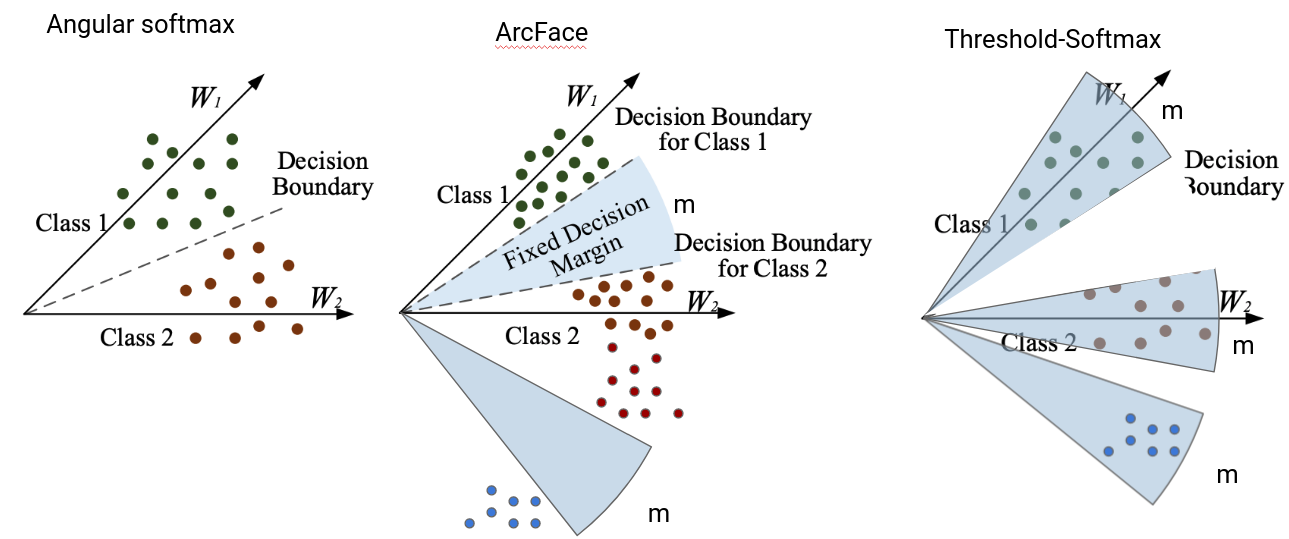
\includegraphics[width=\columnwidth]{50-files/download.png}
    \caption{Comparison of the angular softmax, ArcFace and the proposed Threshold-Softmax. In ArcFace, the margin (in blue) is fixed but the width of the arcs of each class can be arbitrarily wide (or narrow), since there is no constraint on them. In threshold-softmax, there are no enforced margins but the decision boundaries have a fixed width. An artificial class is predicted outside of those trusted cones.}
    \label{fig:tsm}
\end{figure}

ArcFace constrains the representation so that the angular distance to an incorrect class is at least of size $m$, but does not enforce any absolute requirement on the intra-class angles. I wanted to explore the opposite view and constrain the representation vector in the other way, so that the angle between samples of the same class is \emph{at most} $m$, making it an absolute requirement.

I achieved this by concatenating an artificial entry $\cos(m)$ to $\theta$. We say this entry has class $\Omega$. If all the angles in $\theta$ are greater than $m$, then this artificial entry is maxed out by the softmax function, leading to a high loss until the correct angle is finally smaller than $m$. $m$ being a hyperparameter. The loss function can be expressed as:

\begin{equation}
    h(x) = \text{softmax}(s [\cos(f(x),W); \cos m])
\end{equation}

Figure \ref{fig:tsm} highlights the difference with standard angular softmax, ArcFace, and Threshold-Softmax.

\section{Evaluation}

In the subject independent scenario, the dataset LFW \citep{lfw} test set is commonly used to assess the quality of face representation. It consists of 6k image pairs, half being faces of the same identity, half being of different ones. The model has to decide whether a pair of pictures belong or not to the same identity.

State-of-the-art accuracy on this set surpassed 99\% which drove the creation of newer and harder sets.

FGLFW \citep{fglfw} reuses pictures from LFW but selected harder pairs. DeepFace has an accuracy of 92.87\% on LFW but 78.78\% on FGLFW.

The Megaface challenge \citep{megaface} extends this beyond pairs. They propose an input "probe" picture and a gallery of "candidate" pictures. The model has to identify which picture in the gallery is of the same person as the probe.

IJB-{A,B,C} propose a collection of challenges including verification and identification in both pictures and videos.


\section{Extension: Threshold-Softmax with negative samples}

Threshold-Softmax offers us a clear definition of "negative space", aka all vector that the softmax would classify as $\Omega$. This can be naturally leveraged by having "negative samples" (ie samples not belonging to the classes set), and aiming to classify them as class $\Omega$. That way, we can collect cheap samples as this set of negative samples just has to be cleaned of overlaps with the positive samples, and use them as an additional source of supervision. Negative faces might have people looking like some positive identities and the loss would enforce the network to distinguish them so as to place those in the negative space. This is visualized in Figure \ref{fig:neg-tsm}.

\begin{figure}
    \centering
    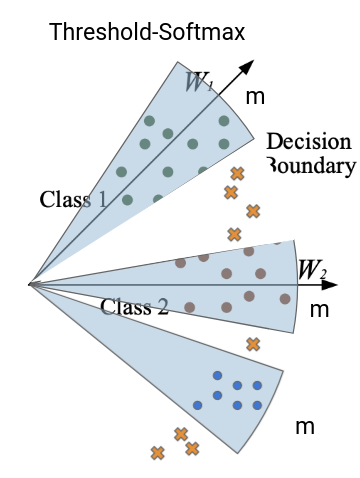
\includegraphics[width=0.25\columnwidth]{50-files/tsm-neg.png}
    \caption{Threshold-softmax with negative samples: crosses are negative samples. We do not know their identities, we just know they do not belong to any of the known identities. Threshold-Softmax naturally uses those samples by placing their identities outside of the known classes decision boundaries, ie, predicting class $\Omega$.}
    \label{fig:neg-tsm}
\end{figure}

\subsection{Experimental study}

We experiment with our new loss function by training on MS1Mv2 and testing on LFW and FGLFW. compare L2-Softmax / Angular Softmax, ArcFace, Threshold-Softmax, Threshold-Softmax with negative samples, at various data availability.

In order to cut training times down, we train on 5\% of the training data for 10 epochs, with a Resnet18 pretrained on ImageNet.

We conduct an experiment with extensive hyperparameter search (for $m$, the learning rate and the weight decay) and sum up our results in Table \ref{tab:tsm-lfw}. In the Threshold-Softmax with negative samples case, we add another 5\% of the dataset with a single negative label. We assess the performance of our proposed loss according to the threshold value in Figure \ref{fig:tsm-angle}.

\begin{table}[]
    \centering
    \begin{tabular}{|c|c|c|}
        \hline
         & LFW & FGLFW \\
        \hline
        L2-Softmax & 97.66 & 88.88 \\
        \hline
        ArcFace & 98.63 & \textbf{95.58} \\
        \hline
        Threshold-Softmax & 98.88 & 93.51 \\
        \hline
        Threshold-SM + Negative & \textbf{98.93} & 95.23 \\
        \hline
    \end{tabular}
    \caption{Accuracy on LFW and FGLFW for various loss functions. Best rejection threshold selected for each method.}
    \label{tab:tsm-lfw}
\end{table}

\begin{figure}
    \centering
    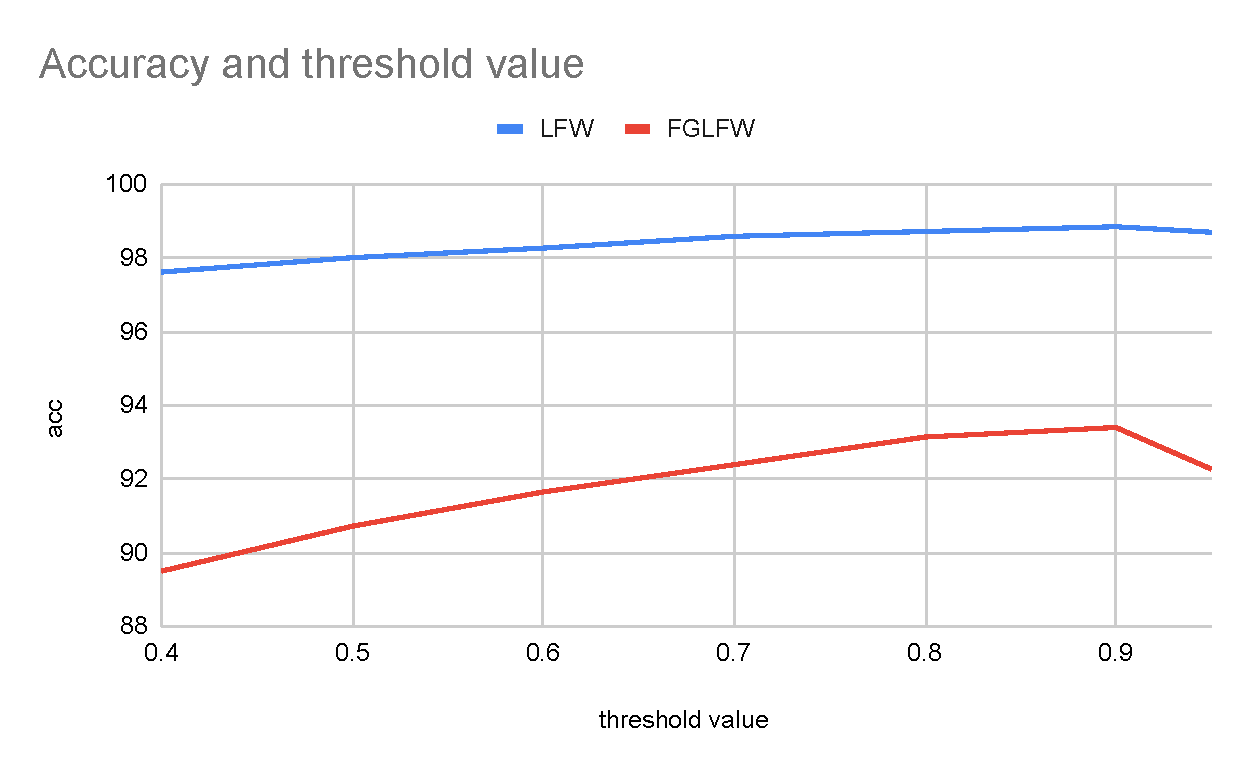
\includegraphics[width=\columnwidth]{50-files/tsm-angle.pdf}
    \caption{Performances on LFW and FGLFW according to the threshold value.}
    \label{fig:tsm-angle}
\end{figure}

We see that the Threshold-Softmax is competitive with ArcFace and better than the raw L2-Softmax. Furthermore, training with negative samples indeed boost the performance of Threshold-Softmax.

Further testing should be conducted with bigger data and epochs budget in order to compare those algorithms in realistic training situations.

It is interesting to note that ArcFace's margin is not mutually exclusive with the cones of trust of Threshold-Softmax and the two could be combined. This is left as future work.

\section{\emph{\arr Contributions}: distractor-robust face recognition for a closed-set of identities}

The following sections will highlight our contributions:

\begin{enumerate}
    \item a comparison of ArcFace and cross-entropy classifiers in the context of closed-set face recognition
    \item a search for a strategy to manually deal with label noise, curate and expend a face recognition dataset for closed-set scenarios
    \item a set of losses and their evaluations allowing to leverage unlabeled negative faces and make face recognition system more robust to distractors. 
\end{enumerate}

\subsection{The limits of metric learning}

Our first attempt of addressing face recognition in our industrial context was based on a publicly available face detection and face recognition pre-trained CNNs. The problem was posed as an open-set face recognition task, and consisted in matching a feature vector extracted from an input photo against each reference image in the database feature vectors, as customary in metric learning. Unfortunately, despite the impressive number, having an accuracy of 99.38\% on LFW means that identifying someone by pair matching among 4000 identities (as we wished initially) triggers 25 positive matches. The performance scored in our setting was substantially worse due to distribution mismatch between the training domain and our application domain.

This shows that the metric learning strategy reached its limits in this setting and is not robust enough to scale to many identities and many distractors. Metric learning aims to learn a powerful embedding function, which is too ambitious for our problem: filtering out distractors, and recognizing a handful of persons of interest. Filtering out distractors better describes the task at hand, allows the net to focus on learning only the facial features for the set of the persons of interest, plus a rejection criterion or margin for rejecting distracting faces.

\begin{figure}
    \centering
    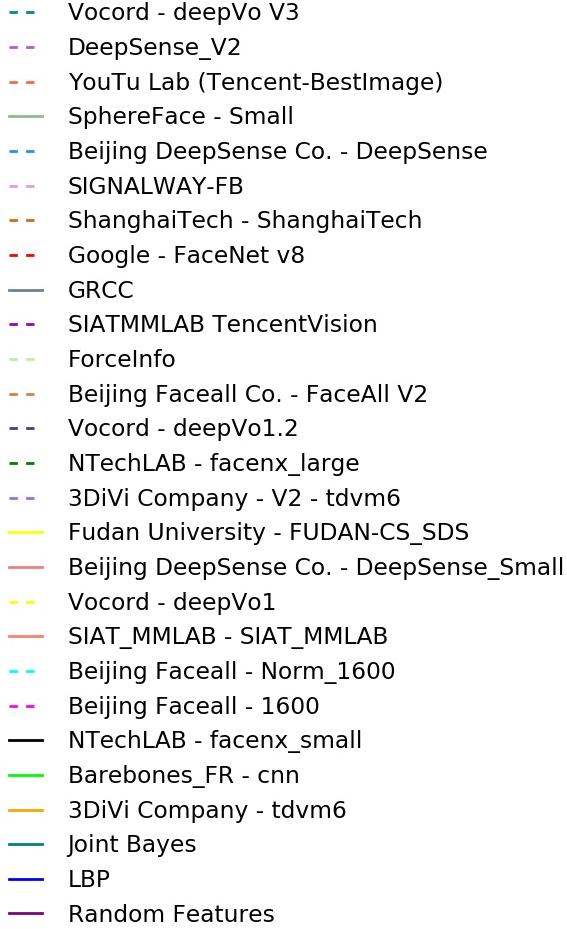
\includegraphics[width=0.3\columnwidth]{50-files/CH1_Legend.png}
    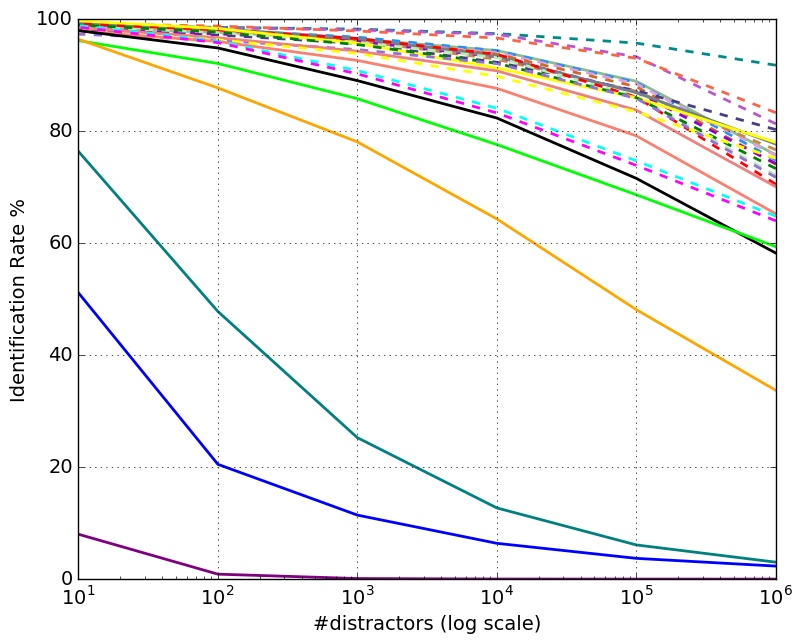
\includegraphics[width=0.45\columnwidth]{50-files/facescrub_rank-1_cmbnd_set_1.jpg}
    \caption{Rank 1 identification performance for contestants on Megaface's Facescrub challenge under various quantities of distractors. Most models have their performance degrading quickly even with 100 distractors only.}
    \label{fig:megafacebad}
\end{figure}

Indeed, Figure \ref{fig:megafacebad} shows that most of the models which participated in the challenge are sensitive to the number of distractors and their performance quickly degrades under 95\%, a threshold under which we consider the models not ready for our application.

\subsection{Back to simple classifiers}

In fact, as the identities to recognize are known ahead of time and part of the training set, it is possible to cast the project as a classification problem, using a regular cross entropy loss. We would be performing the classification from the softmax probabilities, just like the action classification (See \ref{actionclf}).

However, what we miss from such a model is the ability to know when we don't know. This is something modern models are not good at. They tend to be uncalibrated and predict only high confidence scores. \citet{softmaxood} claim that out of domain samples have a lower softmax probability than in distribution samples. This is something we have not observed to be true or sufficient to reliably reject distractors. Moreover, as the nets learn, they tend to overfit the softmax loss and end up predicting higher and higher confidences, even when they're wrong. This makes thresholding the \ac{OoD} rejection confidence score hard as it might change between training runs.

\subsection{Dataset denoising}

We propose a strategy to incrementally clean a dataset from label noise by expending the set of identities to recognize. We explicitly train on negative samples ("distractors") and select a subset of HFaces' identities as a positive training set and the rest as negative set. This allows to grow the positive set in a controlled way, so that the negative set can be denoised progressively. If we had to investigate a classifier among thousands of identities at once, it would be extremely hard to gain insight into the dataset and take actions. Instead, we use as a positive set the top N most popular identities, learn a model, evaluate it, clean or complete the training set, then add another N positive identities when the performances are good for our setting, and iterate.

\subsection{Precision / Recall for dataset construction}

\subsubsection{Motivation}

As the training data can be modified as well in order to address the task, several questions have to be answered in order to grow the dataset in a principled way. Mainly, at any point in time, there are 3 possible situations and their associated response:
\begin{enumerate}
    \item Everything works well enough: grow the set of VIPs
    \item Some VIPs seem to cause too much confusion and trigger too many false positives: rework the data for those identities (looking for errors, low quality or confusing samples) in order to identify harmful samples
    \item Some VIPs are not detected in tests : add samples. Those identities have insufficient data to generalize correctly.
\end{enumerate}

Which one of those actions to take is crucial in order to control the growth of the model and its performance.

\subsubsection{Principles}

\begin{figure}
    \centering
    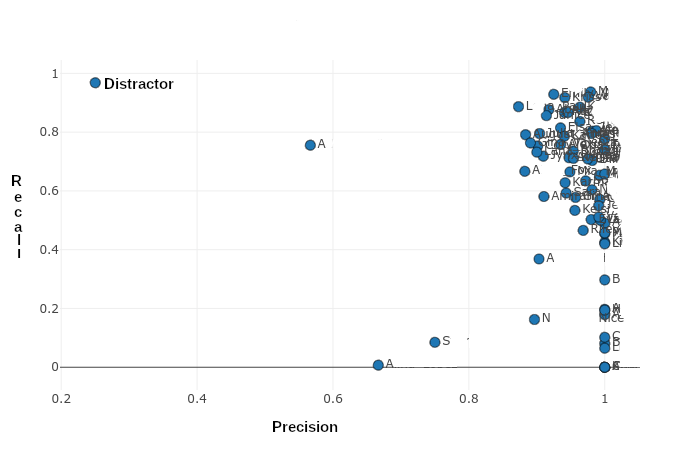
\includegraphics[width=\columnwidth]{50-files/pr-plot.png}
    \caption{Each class (abbreviated to the first letter of the nperson's ame) is placed on this grid depending on its precision and recall scores. Top right is best, bottom left is worst. We aim to find strategies that help moving each point right and up.}
    \label{fig:pr-plot}
\end{figure}


Diagnosing the current state of the dataset in order to choose what to do next happens to be easy thanks to simple metrics. By computing precision / recall by class we get a view of the model performance. In order to easily visualize which class need work, we plot each class on a grid, seen in Figure \ref{fig:pr-plot}. We empirically hypothesize that classes with low precision suffer from noisy training data and/or labels, while classes with low recall indicate a lack of training data.

These assumptions brings insight into the model's state, is easy to implement, interpret and use but bears the drawback that some additional effort must be taken in order to build a meaningful test set for each identity. As we observe strong outliers on the precision/recall plots while building the dataset, we hypothesize that the performance across identities is not correlated (or not enough), and therefore we believe we cannot use a random subset of identities to estimate the overall performance.

In our situation, we accept trading recall for precision as false positives damage the user experience with erroneous suggestions or search results. With false negatives, no labeling is performed, and the user browsing is not impacted.

\subsubsection{Results}

In order to investigate these hypotheses, we select a class which performs well in both precision and recall and run three experiments:

\begin{enumerate}
    \item A base run gives 94\% precision and 99\% recall.
    \item We subtract 50\% of the training data for that class, obtaining 98\% precision and 86\% recall. Here, it is clear that removing data deteriorates recall. By reducing the amount of training data, the identity is more narrowly represented, thus less sensible to accept other faces as belonging to it: the precision slightly increases.
    \item We introduce label noise by integrating someone else's samples into this class' training data. We obtain 94\% precision and 98\% recall.
\end{enumerate}

This data point seem to suggest that recall indeed correlates with the amount of data for a class. Unfortunately, precision does not negatively correlate with label noise. The classifier seems to overfit the noise rather quickly and learn a multimodal class. The question of detecting noisy classes remains unanswered by this approach.

\subsection{Experiments}

\begin{figure}
    \centering
    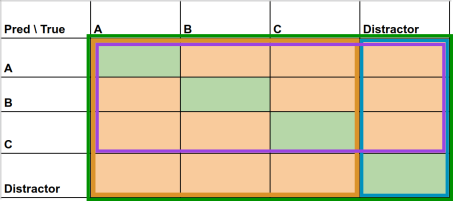
\includegraphics[width=0.6\columnwidth]{50-files/cm.png}
    \caption{We compute some metrics by selecting various meaningful subsets from the confusion matrix: \textcolor{blue}{distractor accuracy} (blue), \textcolor{orange}{identification accuracy} (orange), \textcolor{violet}{kept accuracy} (violet), and \textcolor{ForestGreen}{total accuracy} (green). For each subset, the metric is computed as the sum of the green cells it contains divided by the sum of all cells it contains. A, B, and C are three fictitious identities for illustration purposes}
    \label{fig:cm-metrics}
\end{figure}

We devise a set of experiments in order to evaluate the progress done on the task of face recognition on HFaces. For each experiment, we measure:
\begin{itemize}
    \item the accuracy on the distractor set: among all distractors how many have been predicted as such, ie, the true rejection rate (See Figure \ref{fig:cm-metrics}).
    \item the identification accuracy: the recognition accuracy among non-distractors (See Figure \ref{fig:cm-metrics}).
    \item the overall accuracy on all test samples (See Figure \ref{fig:cm-metrics}).
    \item the mean of the F1 score of each class
    \item the accuracy of kept (non rejected) predictions. We consider that we reject predictions classified as distractors (See Figure \ref{fig:cm-metrics}). This allows us to evaluate how many false identification will be performed on the platform, and choose our precision / recall tradeoff. 
    \item When techniques give scores with predictions and the model performs reasonably well, wrong predictions are given a lower score and correct prediction a higher score. This allows us to trade precision for recall, as we can find a threshold which rejects predictions with low scores until a chosen true positive ratio. Thus, we also compute the identification and total accuracy for 95\% and 99\% true positives, giving us an estimate of the recall for both test sets at those true positive rate goals.
\end{itemize}

We emphasize the industrial context: this tool is to be used in order to label videos on the customer's platform. As such, it is better not to annotate a video than predict a wrong label. Setting a false acceptance rate of 5\% / 1\% (ie 5\% / 1\% of wrong predicted labels, a precision of 95\% / 99\%), we evaluate the recall by computing the accuracy on the identification set and the entire test set. Results are summarized in Figure \ref{fig:tpr}.

We compare several models: ArcFace, and cross-entropy classifiers. We train a simple classifier (CE) also explore several techniques for exploiting distractors from the training set, and rejecting them at inference:  an extra class for distractors (DCE), maximizing entropy on distractors (ME), minimizing logits on distractors (ZLog). We report, in Table \ref{tab:frmetrics}, the various metrics \emph{at the maximum accuracy}.

\begin{figure}
    \centering
    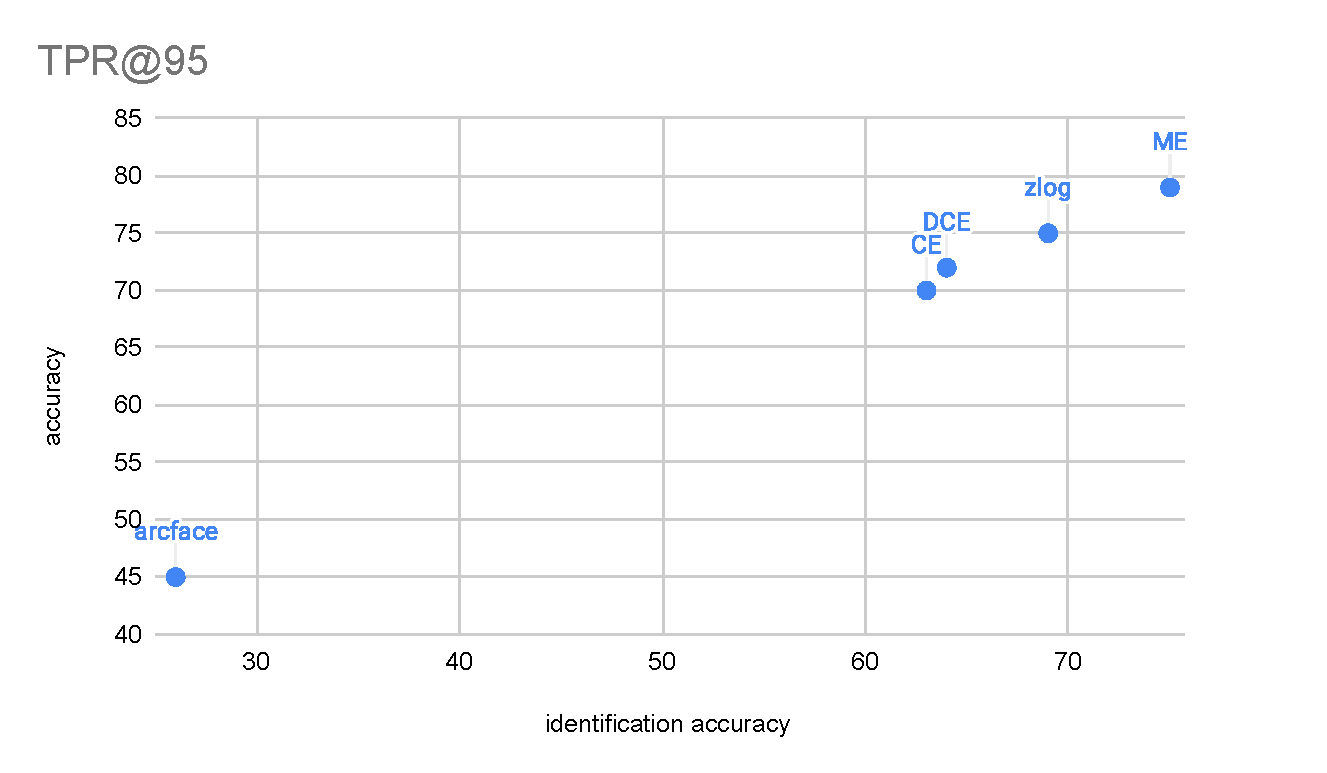
\includegraphics[width=\columnwidth]{50-files/TPR@95.pdf}
    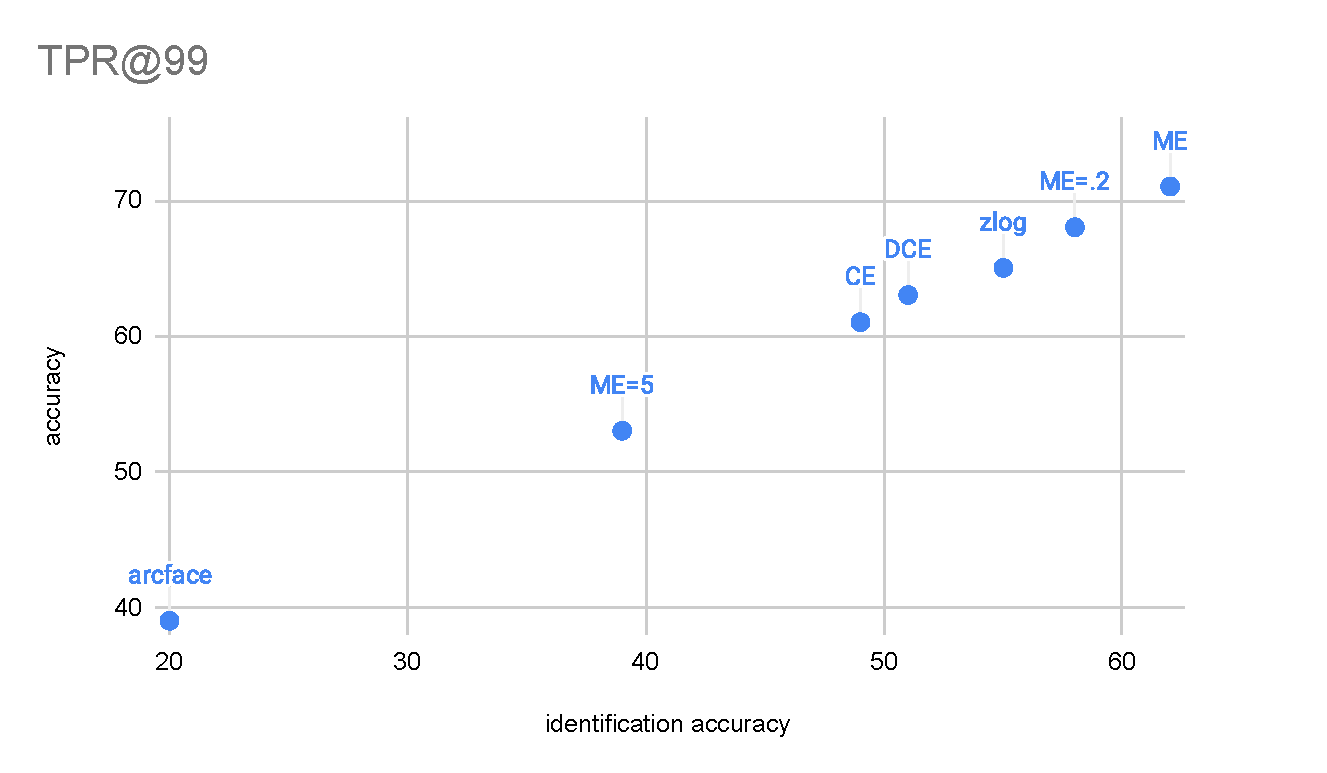
\includegraphics[width=\columnwidth]{50-files/TPR@99.pdf}
    \caption{Identification accuracy and total accuracy for a true acceptance rate of 95\% / 99\%. CE: Cross-Entropy, DCE: Cross-Entropy+Distractors, ME=$x$: Cross-Entropy+MaximumEntropy with maximum entropy weight $x$, zlog=Zero-Logits.}

    \label{fig:tpr}
\end{figure}

\begin{table}[]
    \centering
    \begin{tabular}{|l|c|c|c|c|c|}
    \hline
        Model & distractor     & identification   & total           & mean F1       & kept \\
              & accuracy       &   accuracy       & accuracy        &               & accuracy \\
        \hline
        \hline
        ArcFace & 78.38        & 43.93            & 52.03           & 0.40          & 73.11 \\
        \hline
        CE   & 79.65           & 73.51            & 74.96           & 0.65          & 85.4 \\
        \hline
        DCE & \textbf{95.17}   & 65.35            & 72.36           & 0.62          & \textbf{92.82} \\
        \hline
        ZLog & 79.09          & \emph{78.67}      & \emph{78.77}    & \emph{0.66}   & 84.92 \\
        \hline
        ME & \emph{89.56}     & \textbf{78.93}    & \textbf{81.43}  & \textbf{0.72} & \emph{91.05} \\
        \hline
    \end{tabular}
    \caption{Various metrics for each model, selected at maximal accuracy. CE: Cross-entropy, DCE: Cross-Entropy+Distractors, ME: Cross-Entropy+MaximumEntropy with maximum entropy, ZLog=Zero-Logits. \textbf{Best} and \emph{second best} results are highlighted}
    \label{tab:frmetrics}
\end{table}


\subsubsection{ArcFace}

\begin{figure}
    \centering
    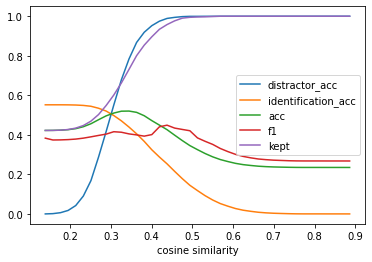
\includegraphics[width=0.45\columnwidth]{50-files/arcface-all.png}
    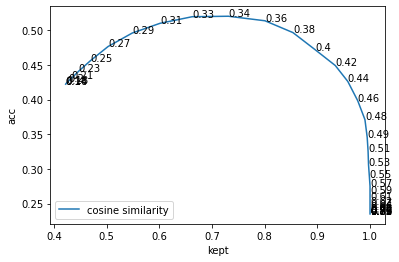
\includegraphics[width=0.45\columnwidth]{50-files/arcface-acc-kept.png}
    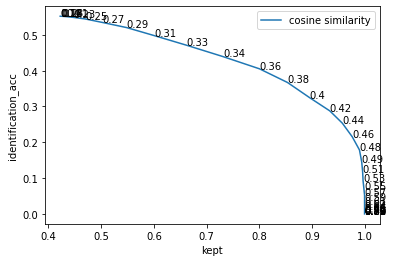
\includegraphics[width=0.45\columnwidth]{50-files/arcface-id-kept.png}
    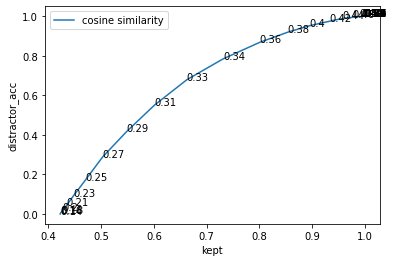
\includegraphics[width=0.45\columnwidth]{50-files/arcface-distr-kept.png}
    \caption{a) Various metrics for the ArcFace model as predictions are set as distractors under various cosine similarity values. b,c,d) As we sweep over the threshold cosine similarity value and reject more samples as distractors, we look at the variations on the metrics against the kept accuracy.}
    \label{fig:arcface-plots}
\end{figure}

We first verify our claim that metric learning is not robust in our setting. We reuse the pretrained ArcFace model published by \url{https://github.com/foamliu/InsightFace-v2}. The important things to note are:

\begin{itemize}
    \item this model has been trained for a face-independent protocol, that is, it has not been trained on the people it was meant to recognize;
    \item this model has several data biases: our distribution includes more females than males, very few above the age of 50. The training set is broader than this narrower distribution of ours. The model is faced with a narrower and more fine-grained task than intended;
    \item Metric learning makes it hard to know when we don't know, thus rejecting distractors is not easy;
    \item ArcFace protocol is about computing the cosine similarity between the representation of the input image and a reference image. For identification, we randomly choose one reference image per class. The choice of that reference image could have been selected against a validation set for minor gains. We made sure that the different metrics do not dramatically change between each run.
    \item We set a distractor threshold. If all reference images have a cosine similarity lower than this threshold, we reject this input as a distractor. We compute our metrics sweeping over threshold values, shown in Figure \ref{fig:arcface-plots}.
\end{itemize}


We get a best accuracy value of 52.3\% for a distractor accuracy of 78\%, an identification accuracy of 44\% and F1 score of 0.40.

\subsubsection{Cross-Entropy (CE)}

\begin{figure}
    \centering
    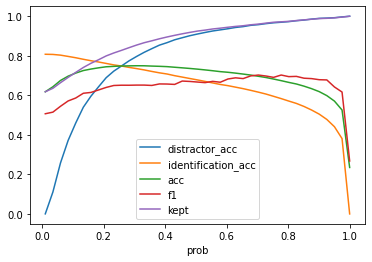
\includegraphics[width=0.45\columnwidth]{50-files/ce-all.png}
    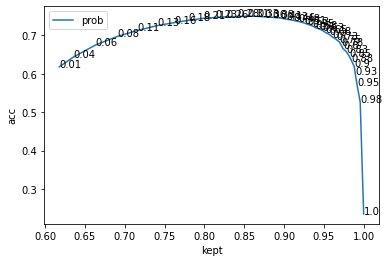
\includegraphics[width=0.45\columnwidth]{50-files/ce-acc-kept.png}
    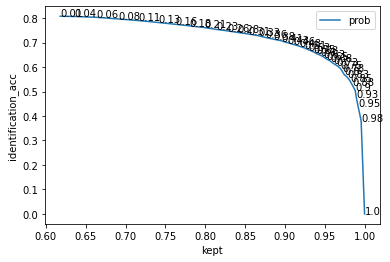
\includegraphics[width=0.45\columnwidth]{50-files/ce-id-kept.png}
    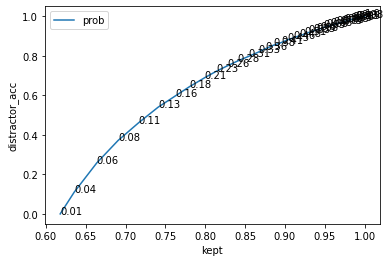
\includegraphics[width=0.45\columnwidth]{50-files/ce-distr-kept.png}
    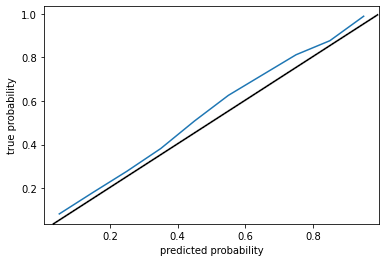
\includegraphics[width=0.45\columnwidth]{50-files/ce-calibration.png}
    \caption{Various metrics for the CE model as predictions are set as distractors under various probability values. Last plot is the network's calibration.}
    \label{fig:ce-plots}
\end{figure}

We now compare the advanced ArcFace loss with a naive softmax+cross entropy loss, trained on the persons of interest only. This model has no built-in way of signaling distractors. We are going to assume that the distractors produce predictions with lower confidence, and threshold on low confidence scores.

Figure \ref{fig:ce-plots} indicates that this heuristic holds some truth. It seems that around 90\% of distractors have a confidence score below 0.25 and half of the people of interest get a confidence score over 0.95. Unfortunately this heuristic is not entirely satisfying. As the rejection threshold increases, the overall accuracy slowly decreases.

It is unsurprising that the base identification accuracy of 81\% is much greater than the 55\% of ArcFace. This model gets a peak accuracy of 75\%, for a distractor accuracy of 80\%, an identification accuracy of 73\%, and a F1 score of 0.65. This model is already indisputably more suited for our task.

\subsubsection{Cross-Entropy with Distractors (DCE)}

\begin{figure}
    \centering
    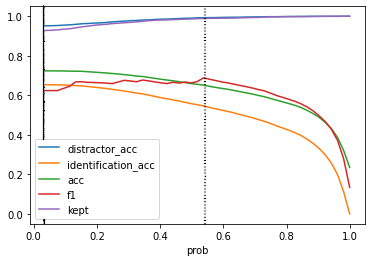
\includegraphics[width=0.45\columnwidth]{50-files/dce-all.png}
    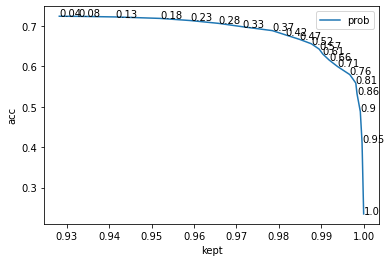
\includegraphics[width=0.45\columnwidth]{50-files/dce-acc-kept.png}
    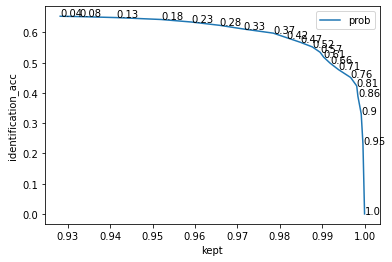
\includegraphics[width=0.45\columnwidth]{50-files/dce-id-kept.png}
    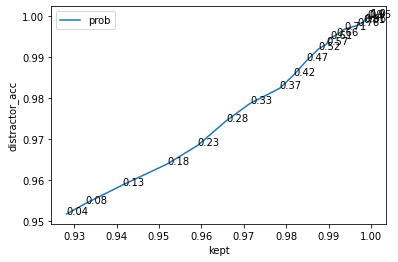
\includegraphics[width=0.45\columnwidth]{50-files/dce-distr-kept.png}
    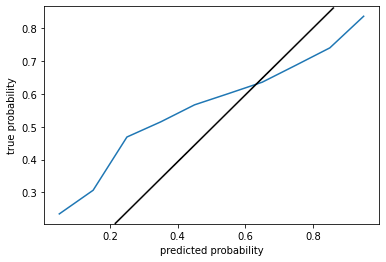
\includegraphics[width=0.45\columnwidth]{50-files/dce-calibration.png}
    \caption{Various metrics for the DCE model as predictions are set as Distractors under various probability values.}
    \label{fig:dce-plots}
\end{figure}


Aiming to improve both the representational power of our model and teaching it the ability to reject distractors, we add distracting faces to our training data that have to be classified as their own distractor class. Similarly to the previous model, we evaluate how the different metrics behave when we also consider as distractors predictions below a given threshold in Figure \ref{fig:dce-plots}. The peak accuracy of 72\% is below the one of the simple classifier, explained by a lower ability to recognize the people of interest (from 73\% to 65\%) but a much greater ability to detect distractors (from 80\% to 95\%). Overall the models have a comparable F1 score of 0.62. However, the model behaves better in our industrial scenario, as shown in Figure \ref{fig:tpr}.

\subsubsection{Cross-Entropy + ZeroLogits (zlog)}

\begin{figure}
    \centering
    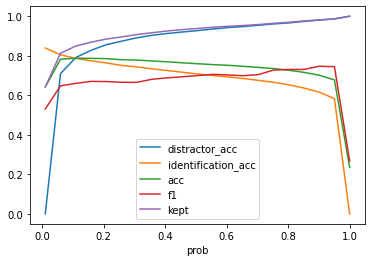
\includegraphics[width=0.45\columnwidth]{50-files/zlog-all.png}
    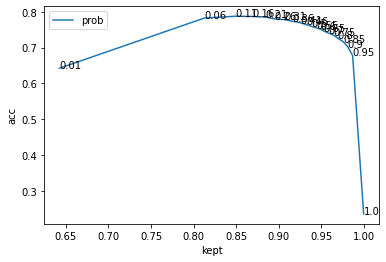
\includegraphics[width=0.45\columnwidth]{50-files/zlog-acc-kept.png}
    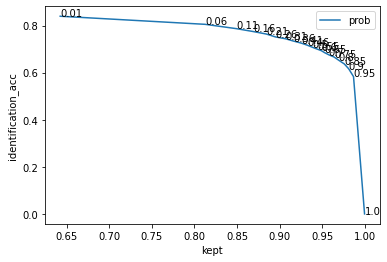
\includegraphics[width=0.45\columnwidth]{50-files/zlog-id-kept.png}
    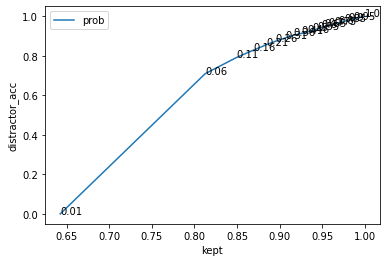
\includegraphics[width=0.45\columnwidth]{50-files/zlog-distr-kept.png}
    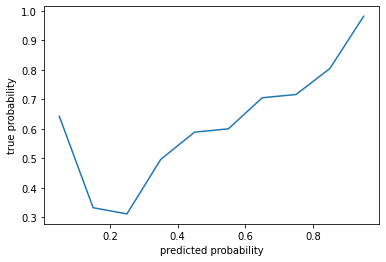
\includegraphics[width=0.45\columnwidth]{50-files/zlog-calibration.png}
    \caption{Various metrics for the zlog model as predictions are set as Distractors under various probability values.}
    \label{fig:zlog-plots}
\end{figure}

Inspired by \citet{goodosr}, we hypothesize that distractors can be sorted by a lower logit value than persons of interest. Distractors are not their own class anymore, but are discriminated from the low logits they produce. We propose penalize their square logits, further encouraging them to zero, and classify only the persons of interest with a cross-entropy loss.

We find that this brings some improvements in identification accuracy and total accuracy, bringing the F1 score to 0.66. This model also performs better when fixing the true positive rate.

However, contrarily to \citet{goodosr} we don't observe logits to be more informative than softmax probabilities. We tried thresholding distractors with logits in each model, every time bringing equivalent or lower results. For this reason, we do not report those results.

\subsubsection{Cross-Entropy + Maximum Entropy (ME)}

\begin{figure}
    \centering
    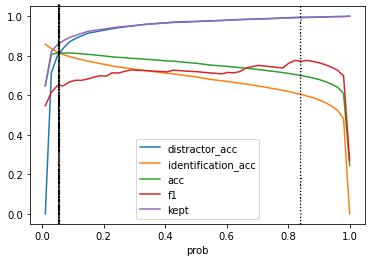
\includegraphics[width=0.45\columnwidth]{50-files/me-all.png}
    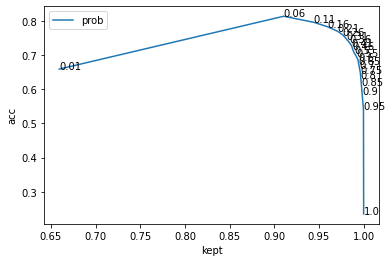
\includegraphics[width=0.45\columnwidth]{50-files/me-acc-kept.png}
    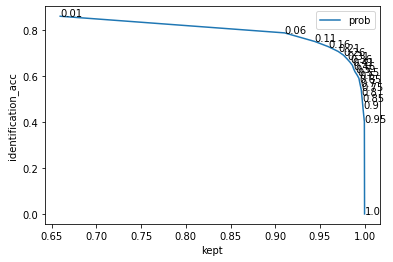
\includegraphics[width=0.45\columnwidth]{50-files/me-id-kept.png}
    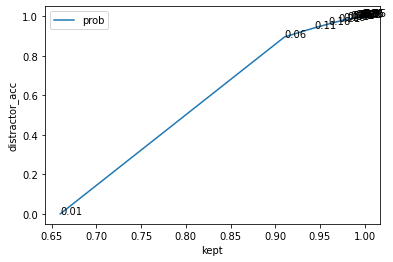
\includegraphics[width=0.45\columnwidth]{50-files/me-distr-kept.png}
    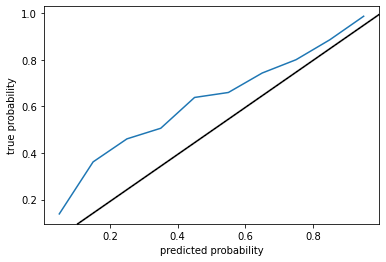
\includegraphics[width=0.45\columnwidth]{50-files/me-calibration.png}
    \caption{Various metrics for the ME model as predictions are set as distractors under various probability values.}
    \label{fig:me-plots}
\end{figure}

Finally, observing that the zlog model was not working as well on logits than on probabilities, despite the loss working directly with them, we envision working on probabilities. Model CE shows that distractors naturally produce lower probabilities, so we aim to predict a maximum entropy (flat) distribution for distractors.

We evaluate this model with weights 1, 5, 0.2 on the maximum entropy loss. A weight of 1 brings the best results, shown in Figure \ref{fig:me-plots}.

\subsubsection{Discussion}

Overall, the ME approach results in the best way to leverage distractors in order to build our industrial system, as can be seen on the TPR plots. It results in the best total and identification accuracy and F1, while being the runner up in kept accuracy. The ZLog technique scores second but is inferior in every way.

The DCE method attracts our attention as well, scoring the highest distractor accuracy and kept accuracy. However, its identification and total accuracy, as well as its F1 are the lowest among the cross-entropy classifier. We conclude that this strategy just over emphasizes classifying as distractor, decreasing identification recall too strongly. Being only 1\% lower in kept accuracy, the ME is a better compromise as we will have a slightly higher error \emph{ratio} but predict a much higher \emph{number} of correct predictions.

\section{Conclusion}

We showed that off-the-shelf  face recognition classifiers, trained with ArcFace, were not satisfying for our industrial scenario. We first explored remaining in the Metric Learning realm and proposed the Threshold-Softmax loss function that is able to use negative samples that are cheaper to collect. However, Threshold-Softmax remains a technique for subject-independent face verification and indentification.

We moved away from metric learning and went back to classifier as our system only has to recognize identities known ahead of time, in a subject-dependent, open-set fashion. We explored various ways of making it robust to distractors, unknown people that the system must learn to discriminate. We explored various techniques to reject distractors at inference time and use distractors at training time, and found that maximizing the entropy for distractors to be the best performing strategy we tried. It is used in production today.

We search for a principled way to refine and extend the training set, leveraging precision/recall plots. While our hypothesis on recall looks promising, we still don't know how to manipulate precision and our hypothesis has been disproved.

The final system is currently used in production, labeling 15k videos a day, and the extracted labels are used as planned to enrich the user experience.

% FIXME grouper par figure plutôt qu'xp